\documentclass[12pt,a4paper]{amsart}

% ukazi za delo s slovenscino -- izberi kodiranje, ki ti ustreza
\usepackage[slovene]{babel}

%\usepackage[T1]{fontenc}
\usepackage[utf8]{inputenc}
\usepackage{amsmath,amssymb,amsfonts}
\usepackage{url}
%\usepackage[normalem]{ulem}
\usepackage[dvipsnames,usenames]{color}
\usepackage{verbatim}

\usepackage{graphicx}
\graphicspath{ {./images/} }



% ne spreminjaj podatkov, ki vplivajo na obliko strani
\textwidth 15cm
\textheight 24cm
\oddsidemargin.5cm
\evensidemargin.5cm
\topmargin-5mm
\addtolength{\footskip}{10pt}
\pagestyle{plain}
\overfullrule=15pt % oznaci predlogo vrstico


% ukazi za matematicna okolja
\theoremstyle{definition} % tekst napisan pokoncno
\newtheorem{definicija}{Definicija}[section]
\newtheorem{primer}[definicija]{Primer}
\newtheorem{opomba}[definicija]{Opomba}

\renewcommand\endprimer{\hfill$\diamondsuit$}


\theoremstyle{plain} % tekst napisan posevno
\newtheorem{lema}[definicija]{Lema}
\newtheorem{izrek}[definicija]{Izrek}
\newtheorem{trditev}[definicija]{Trditev}
\newtheorem{posledica}[definicija]{Posledica}


% za stevilske mnozice uporabi naslednje simbole
\newcommand{\R}{\mathbb R}
\newcommand{\N}{\mathbb N}
\newcommand{\Z}{\mathbb Z}
\newcommand{\C}{\mathbb C}
\newcommand{\Q}{\mathbb Q}

% ukaz za slovarsko geslo
\newlength{\odstavek}
\setlength{\odstavek}{\parindent}
\newcommand{\geslo}[2]{\noindent\textbf{#1}\hspace*{3mm}\hangindent=\parindent\hangafter=1 #2}

% naslednje ukaze ustrezno popravi
\newcommand{\program}{Matematika z računalnikom} % ime studijskega programa: Matematika/Finan"cna matematika
\newcommand{\imeavtorja}{Jan Založnik in Mai Praskalo} % ime avtorja
\newcommand{\imementorja}{} % akademski naziv in ime mentorja
\newcommand{\naslovdela}{}
\newcommand{\letnica}{2022} %letnica diplome


% vstavi svoje definicije ...




\begin{document}

% od tod do povzetka ne spreminjaj nicesar
\thispagestyle{empty}
\noindent{\large
UNIVERZA V LJUBLJANI\\[3mm]
FAKULTETA ZA MATEMATIKO IN FIZIKO\\[2mm]
% FAKULTETA ZA RAČUNALNIŠTVO IN INFORMATIKO\\[2mm]
GEN-I\\[5mm]
% \program\ -- 2.~stopnja}
\vfill

\begin{center}{\large
\imeavtorja\\[2mm]
% {\bf \naslovdela}\\[10mm]
{\bf Uporaba metod strojnega učenja za napoved gibanja cen posameznih urnih blokov}\\[1cm]
%Mentor: \imementorja}
}
\end{center}
\vfill

\noindent{\large
Ljubljana, \letnica}

\pagebreak

\section{Motivacija}

Električno energijo je v primerjavi z ostalimi energenti in dobrinami zelo zahtevno shranjevati, 
zato morata biti proizvodnja in poraba električne energije konstantno v ravnovesju.
Tržni igralci tako izravnavajo svojo proizvodnjo in porabo na znotrajdnevnih trgih električne energije,
kjer se trguje elektrika za dobavo v posameznih 15 minutnih blokih do vsega nekaj minut pred začetkom 
dobave. V zadnjih letih se je predvsem zaradi rasti deleža proizvodnje elektrike iz obnovljivih virov, 
ki je zaradi odvisnosti od vremena težko napovedljiva, dejavnost na znotrajdnevnih trgih močno povečala, 
igralci na teh trgih pa vedno večji delež odločitev prepuščajo umetni intelegenci.



\section{Naloga}

Pri nalogi bova s pomočjo metod strojnega učenja napovedala gibanje cen posameznih urnih
 blokov. Pri tem bova uporabila pretekle podatke o gibanju cen elektrike kot tudi ostalih energentov, 
 vremenske napovedi različnih ponudnikov, podatke o proizvodnji različnih elektrarn itd. 

Najina glavna naloga je ustvariti program, ki bo sprejel zgodovinske podatke o vremenu, cene posameznih
 blokov dnevnega (angl. \textit{day-ahead}) trga ter cene drugih energentov in bo s pomočjo teh poskušal čim bolje napovedati ceno na pripadajočem znotraj dnevnem (angl. \textit{intra-day}) trgu. 
 Za začetek bova opravila analizo podatkov, cena iz dnevnega trga predstavlja že nek začetni približek cen na znotraj dnevnem trgu, zato bova to vzela kot osnovno napoved, ki jo bova skušala izboljšati.



\section*{Električni trg}

V ekonomskem smislu je elektrika surovina, s katero je mogoče trgovati na trgu električne energije \textbf{PX} (angl. \textit{Power Exchange}). Kot je že bilo rečeno je električno energijo zelo težko shranjevati in hkrati morata biti proizvodnja in poraba neprestano v ravnovesju.
 Na trgu dobimo pošteno ceno z načelom ponudbe in povpraševanja, kar pomeni, da proizvajalci podajo ponudbo (koliko električne energije lahko proizvedejo in za kakšno ceno), nasprotno porabniki električne energije podajo povpraševanje (koliko električne energije bodo porabili in koliko so zanj pripravljeni plačati). 
Tako dobimo dve krivulji in stičišče teh predstavlja ceno elektrike, kar prikazuje slika \ref{fig:postena_cena}. \begin{comment}V praksi se tako določi tako imenovani ``day-ahead`` in ``intra-day`` ceni.\end{comment} Zavedati se moramo, da so na trgu mogoče tudi negativne cene.
 Negativne cene so cenovni signal na veleprodajnem trgu električne energije, ki se pojavi, ko visoka nefleksibilna proizvodnja električne energije zadovolji nizko povpraševanje. Neprilagodljivih virov energije ni mogoče hitro in stroškovno učinkovito izklopiti in znova zagnati. Prav tako je cenovno zahtevno zaustaviti obnovljive vire energije.  
 Cene padajo z nizkim povpraševanjem in signalizirajo generatorjem na zmanjšanje proizvodnje, da se izognejo preobremenitvi omrežja. Na dnevnem in znotraj dnevnem trgu lahko tako cene padejo pod ničlo.

\begin{figure}[h]
    \centering
    \includegraphics[scale=0.75]{curve}
    \caption{Graf ponudbe in povpreševanja}
    \label{fig:postena_cena}
\end{figure}
\begin{comment} 
V Evropi imamo več različnih električnih trgov, največja sta Nord Pool (v 16 državah) in Epex Spot (v 13 državah), vendar Slovenija ni del nobenega od teh. 
Povezovanje evropskih trgov omogoča prost pretok električne energije čez meje, kar poveča konkurenčnost na trgu ter s tem dosežemo boljšo učinkovitost. S čezmejnim trgovanjem torej vplivamo na socialno blaginjo vseh Evropejcev.
V najini nalogi se bova osredotočila le na 
Nemčijo, kjer trgujejo na obeh izmed omenjenih trgov. Prav tako so bile na teh trgih izvedene vse transakcije o trgovanju, ki jih bova uporabila pri analizi in napovedovanju. 





Evropska Unija se zavzema, da se bo delež obnovljivih virov do leta 2030 dvignil iz 25\% na več kot 50\%. Prav tako je cilj, da bo proizvedena zadostna količina energije, ko ne bo vetra in sonca. 
Eden izmed načinov je shranjevanje električne energije, ko veterne in sončne elektrarne pridelajo presežek. 
\end{comment}


\section*{Dnevni in znotraj dnevni trg}

Dnevni trg se upravlja prek dražbe, ki poteka enkrat na dan, skozi celotno leto. Na tej dražbi se trguje za vse ure naslednjega dne. Naročila so prijavljena s strani udeležencev na trgu, 
in sicer imajo udeleženci čas do 12:00 UTC, da oddajo vsa ponudbe in povpraševanja za naslednji dan. Na podlagi nakupnih naročil se vzpostavi krivulja povpraševanja, na podlagi prodajnih naročil pa krivulja ponudbe za vsako uro naslednjega dne. Tržna klirinška cena (MCP), ki odraža ponudbo in povpraševanje, leži na presečišču obeh krivulj.


Na znotraj dnevnem trgu udeleženci trga trgujejo neprekinjeno, 24 ur na dan, z dostavo še isti dan. Takoj, ko se ujemata naročilo za nakup in prodajo, se posel izvede. Z električno energijo je mogoče trgovati do 5 minut pred dostavo in prek urnih, polurnih ali četrturnih pogodb. Ker to omogoča visoko stopnjo prilagodljivosti, člani uporabljajo znotraj dnevni trg za prilagoditve v zadnjem trenutku in za uravnoteženje svojih pozicij bližje dejanskemu času. Čezmejno trgovanje je bistveno pri trgovanju znotraj dneva. 


\begin{comment}
\section*{Nemčija}

Nemčija se je zavezala, da bo do leta 2020 zmanjšala emisije toplogrednih plinov za 40 \% v primerjavi iz leta 1990 in za 80–85 \% do leta 2050 glede na raven iz leta 1990. Da bi dosegla tak cilj, Nemčija načrtuje preoblikovanje svojega sistema oskrbe z električno energijo v električno energijo, ki v celoti temelji na obnovljivih virih energije. Potencial za zmanjšanje emisij v elektroenergetskem sektorju je zelo velik, saj ima energetski sektor ključno funkcijo glede emisij toplogrednih plinov, saj trenutno povzroča več kot 80 \% emisij v Nemčiji in znotraj tega sektorja je oskrba z električno energijo odgovorna za približno 40 \% emisije CO2, povezane z energijo. Z visoko učinkovito rabo električne energije, ki v celoti temelji na obnovljivih virih energije, bo mogoče doseči raven skoraj nič emisij toplogrednih plinov.
Zanimiva je tudi porazdelitev nemških električnih virov, ki je prikazana na sliki \ref{fig:distribution}. Hitro se lahko opazi, da velik delež predstavljata veterna in sončna energija, ki pa sta seveda zelo odvisna od vremena.
\end{comment}

\begin{comment}
\begin{figure}[h]
    \centering
    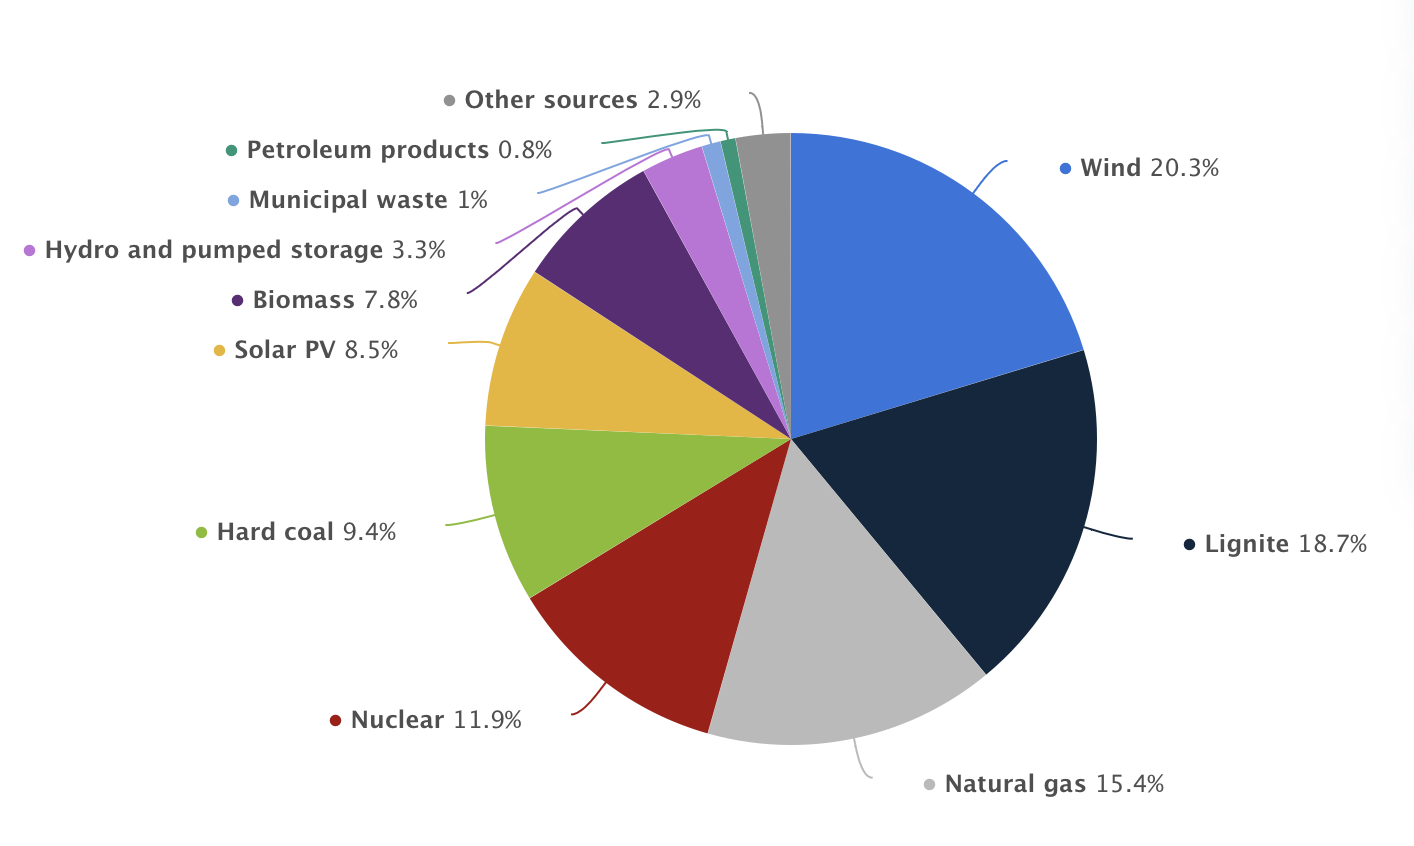
\includegraphics[scale=0.5]{porazdelitev_germany_2021.png}
    \caption{Porazdelitev nemških električnih virov v letu 2021}
    \label{fig:distribution}
\end{figure}
\end{comment}


\section*{Vremenski podatki}

Vremenske podatke bova pridobila iz Evropskega centera za srednjeročne vremenske napovedi (ECMWF). Kot sva že omenila, bo imelo vreme zaradi vedno večjega deleža obnovljivih virov vedno večji vpliv na cene in proizvajanje elektrike. 
Največji delež obnovljivih virov sta v letu 2021 predstavljala veter in sončna energija, zato bova za napoved proizvedene energije uporabila veterne in sončne napovedi iz ECMWF.
\begin{comment} 
Da bi bila ocena čim bolj natančna bova upoštevala dejstvo, da je na severu Nemčije veliko več veternih elektrarn kot na jugu (Slika \ref{fig:veter}).  
Sončne elektrarne so porazdeljene bolj enakomerno (slika \ref{fig:sonce}).
\end{comment}

\begin{comment}
\begin{figure}[h]
    \centering
    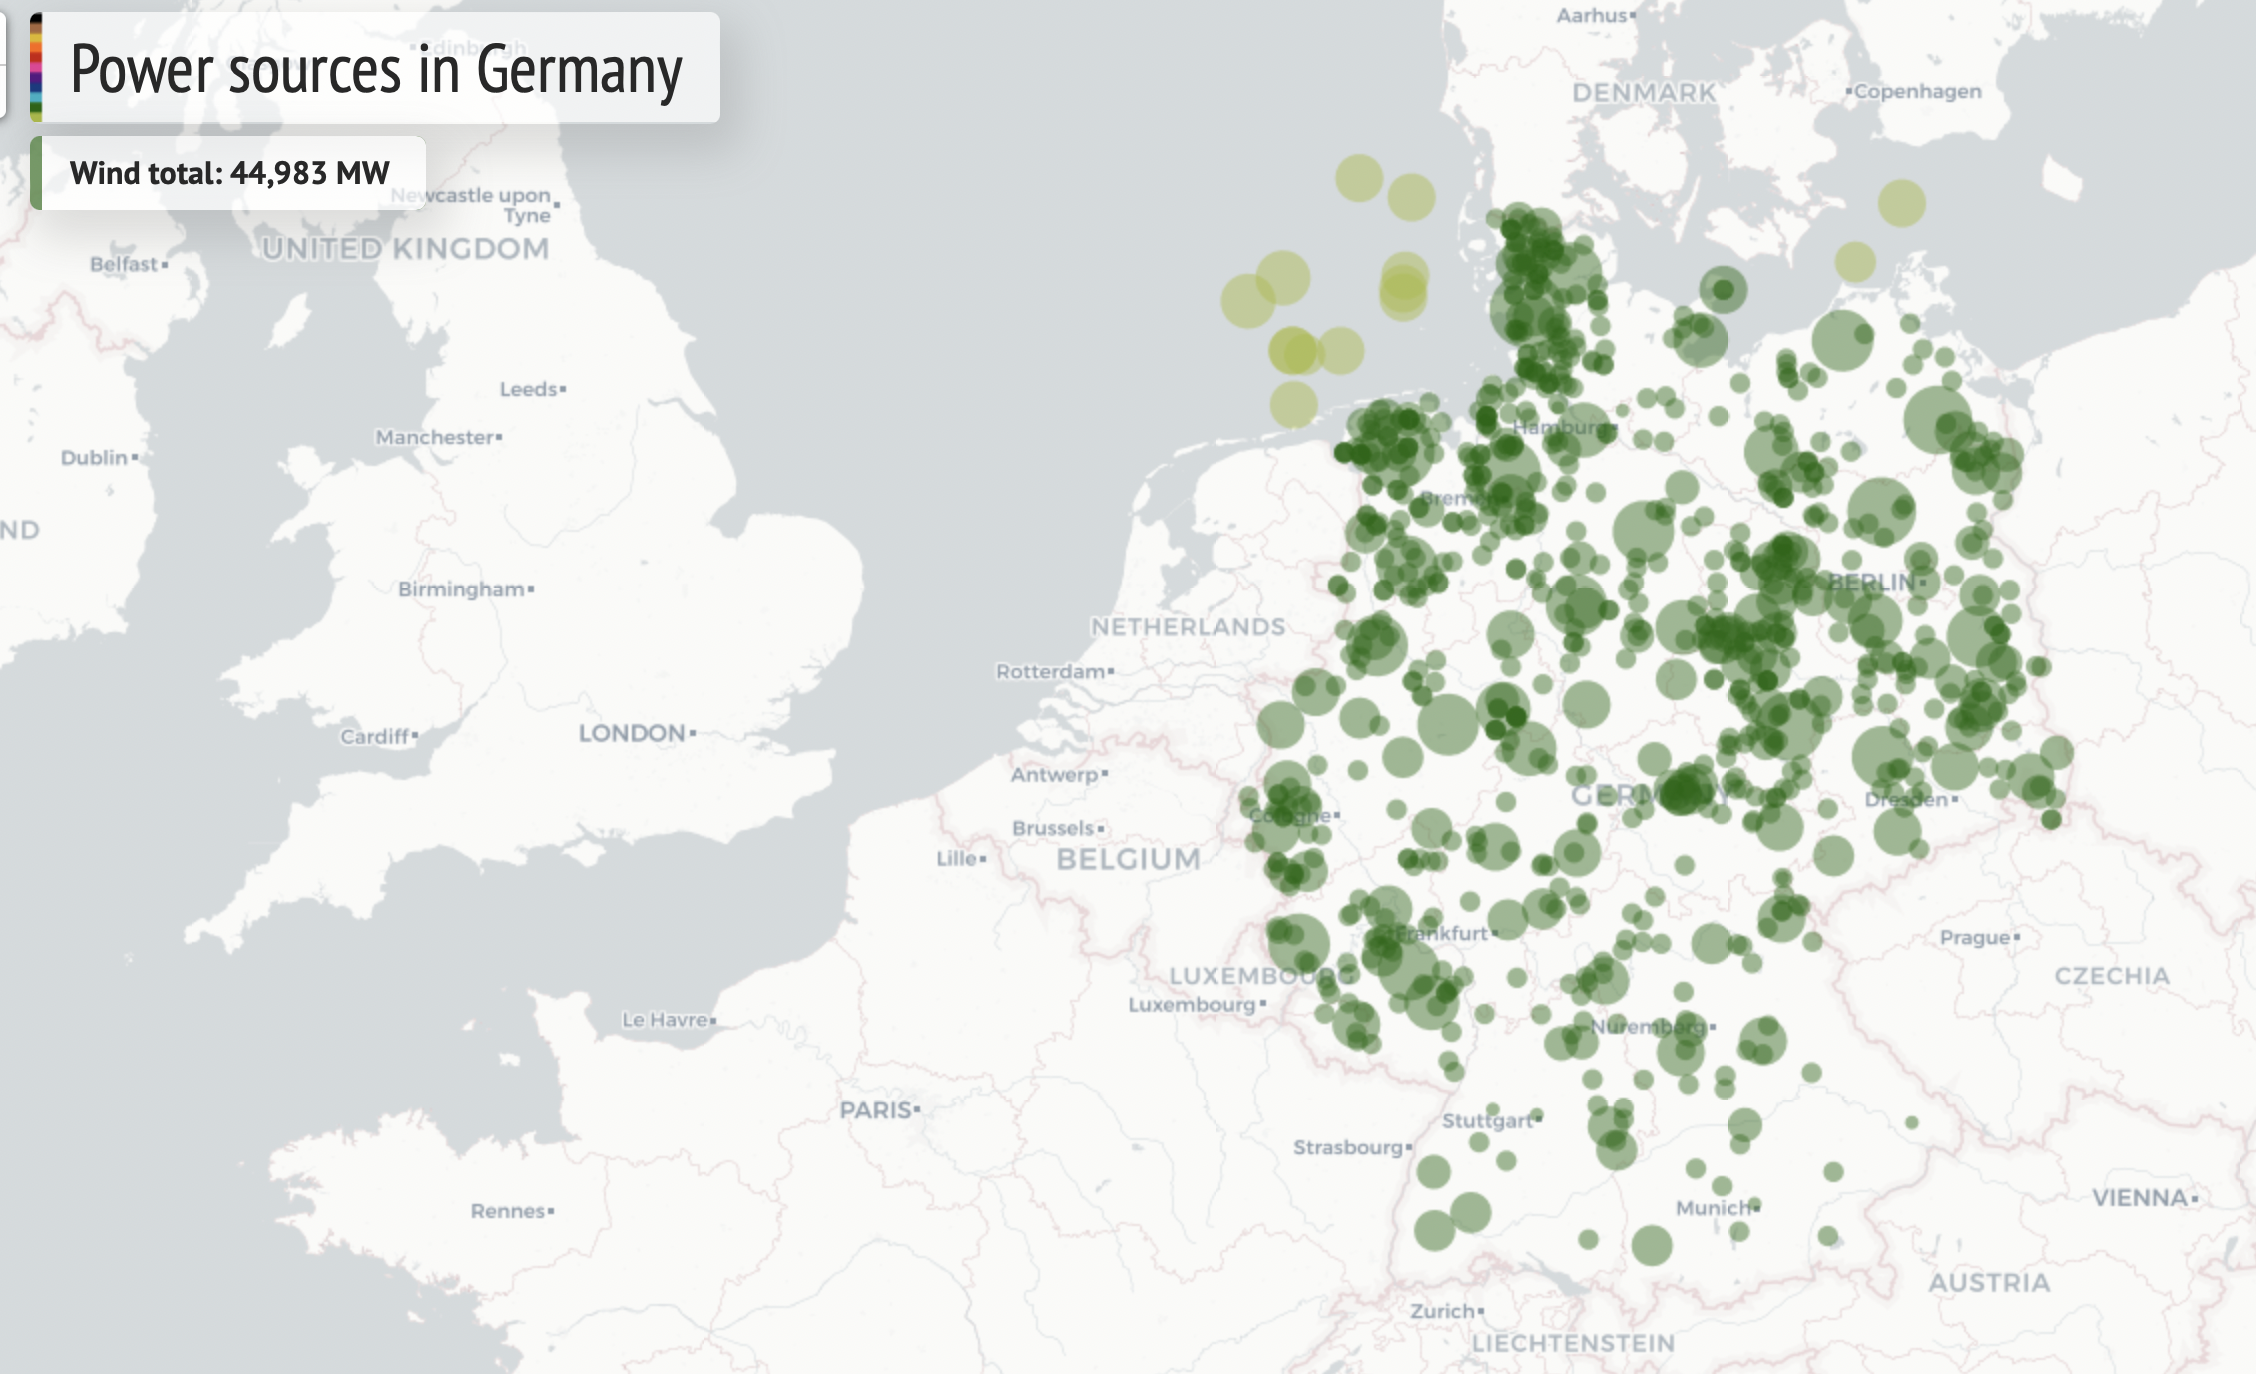
\includegraphics[scale=0.25]{wind_2016.png}
    \caption{Vetrne elektrarne v Nemčiji}
    \label{fig:veter}
\end{figure}

\begin{figure}[h]
    \centering
    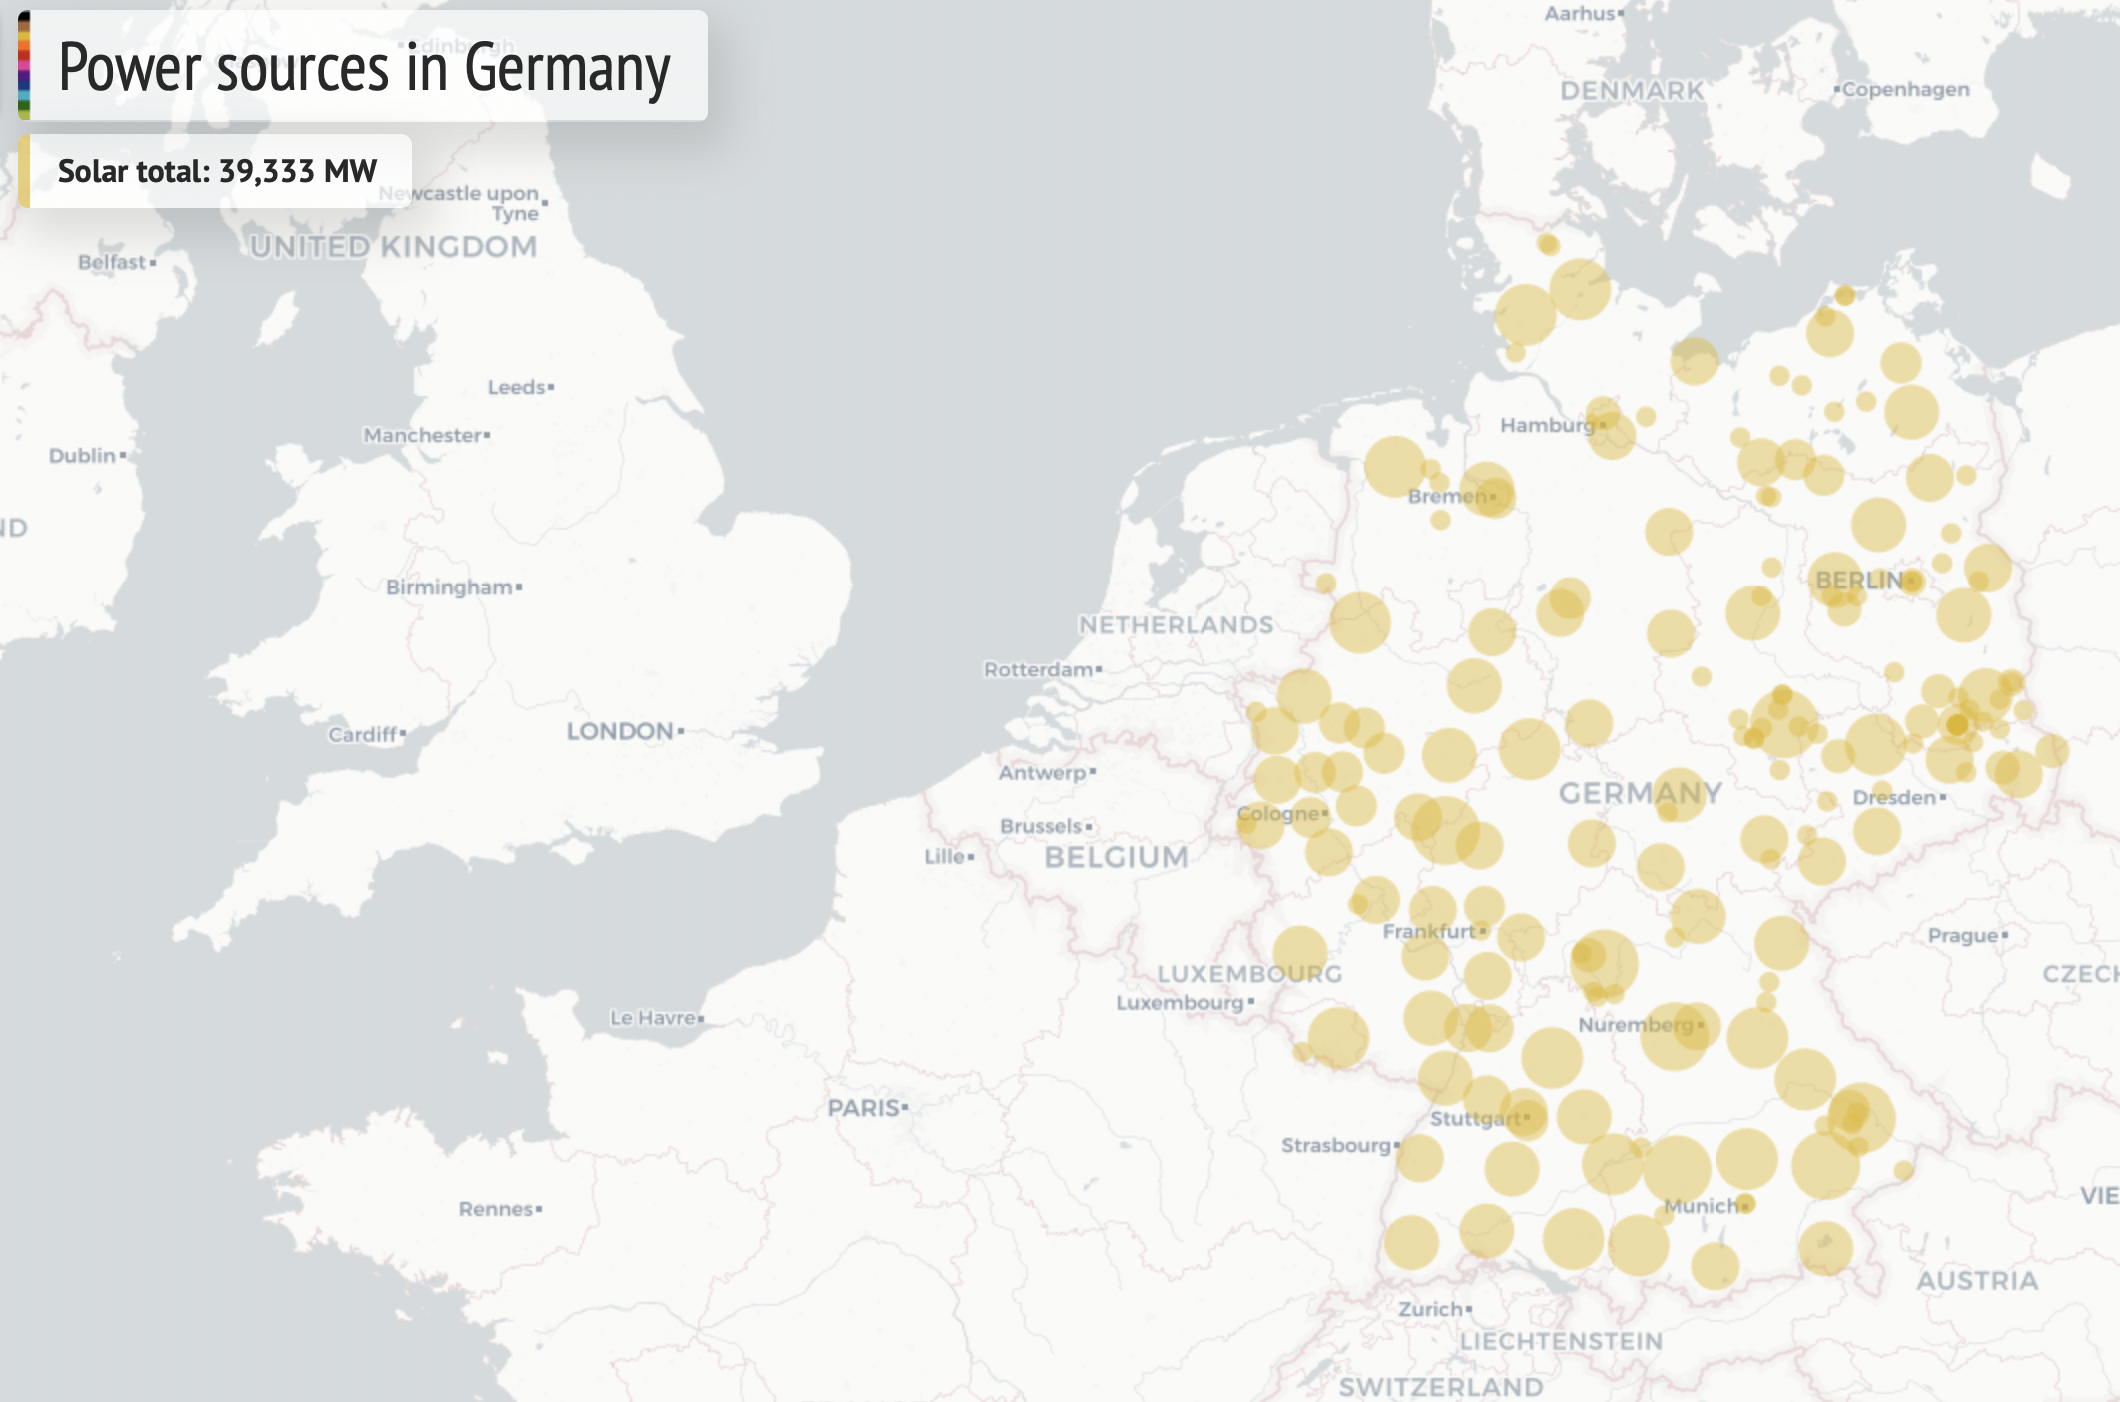
\includegraphics[scale=0.25]{solar_2016.png}
    \caption{Sončne elektrarne v Nemčiji}
    \label{fig:sonce}
\end{figure}
\end{comment}





% možne negativne cene
%amerika in druge ------ Evropa 
% najina ciljna država bo nemčija 
% pomembne so tut strukture kak kdo dobi elektriko
%več je obnovljive in je bolj volatilna cena
% Vreme
%uravnovešanje elektrike da je skos v ravnotežju



% linki:

% https://www.carbonbrief.org/how-germany-generates-its-electricity

%\subsection*{Evropa}

%\subsection*{Druga tržišča}
%\pagebreak
\section*{Podatki o cenah na dnevnem in znotraj dnevnem trgu}
Zaradi nedostopnosti podatkov tako dnevnega in znotraj dnevnega bodo ti pridobljeni iz strani GEN-I. Posamezni trgi sicer ponujajo podatke in programske vmesnike za delo z njimi, a so le-ti plačjivi.


\begin{comment}
\pagebreak


\section*{Projekt}

V nadaljevanju bova s pomočjo LSTM (ali mogoče katerega drugega) modela poskušala napovedati ceno na ``day-ahead`` trgu za naslednji dan in tudi kakšnemu trendu bo sledila ``intra-day`` cena. Kot na vseh drugih trgih je tudi tukaj možen zaslužek s pravo strategijo. Najin cilj je s pomočjo vremenskih podatkov čimbolje napovedati gibanje cene elektrike. 
\end{comment}


\end{document}
